\usetikzlibrary{backgrounds}

\vspace*{-2.3cm}\hspace{8cm}%
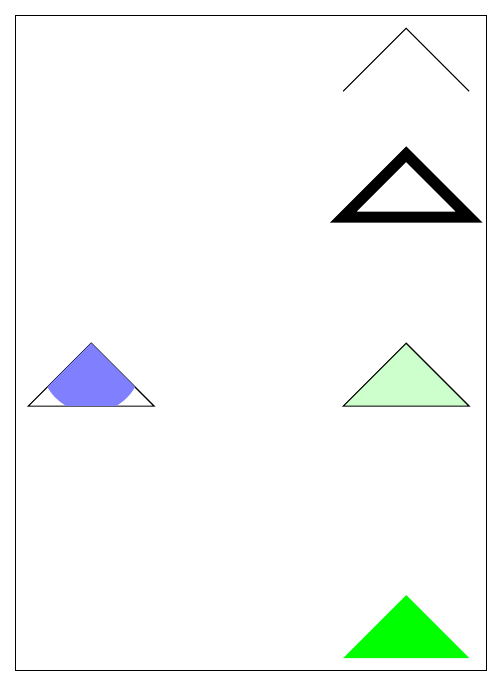
\begin{tikzpicture}[ scale=.8, show background rectangle]

\path[draw] (1,6) -- (2,7) -- (3,6);


\path[draw,line width=4pt] (1,4) -- (2,5)--(3,4)--cycle;

\path[draw, fill=green!20] (1,1)--(2,2)--(3,1)--cycle;


\path[fill=green] (1,-3) -- (2,-2) -- (3,-3) -- cycle;


\path[clip, draw] (-4,1)--(-3,2)--(-2,1)--cycle;
\path[fill=blue!50] (-3, 1.7) circle (.8);





\end{tikzpicture}